\documentclass[10pt]{article}
\usepackage[]{ragged2e}
\usepackage{fancyhdr,amsmath,amsthm,amssymb,bbm,tensor,graphicx}
\usepackage[utf8]{inputenc}
\usepackage[letterpaper,left=25mm,right=25mm]{geometry}

\setlength{\parskip}{1em}
\setlength{\parindent}{0em}

\newcommand{\Z}{\mathbb{Z}}
\newcommand{\R}{\mathbb{R}}
\newcommand{\Q}{\mathbb{Q}}
\newcommand{\C}{\mathbb{C}}
\newcommand{\N}{\mathbb{N}}
\newcommand{\Sp}{\mathbb{S}}
\newcommand{\Pro}{\mathbb{P}}
\newcommand{\dif}{\text{d}}
\newcommand{\di}[2][]{\frac{\partial #1}{\partial #2}}
\newcommand{\del}[2][]{\frac{d #1}{d #2}}

\DeclareMathOperator{\Ima}{Im}
\DeclareMathOperator{\cotan}{cotan}

\linespread{1.25}
\pagestyle{fancy}
\fancyhf{}
\lhead{PHYS 476 $|$  Assignment 3}

\rhead{Dilraj Ghuman $|$ 20564228}

\begin{document}

\textbf{Question 1}

\textbf{(a)} First, we recall that the stress energy tensor for a perfect fluid is
\[ T_{ab} = (\rho + p)u_{a}u_{b} + pg_{ab} \, .\]
So, we are assuming that $p = w \rho$, thus this becomes
\[ T_{ab} = (\rho + w \rho)u_{a}u_{b} + w\rho g_{ab} = \rho\left((1 + w)u_{a}u_{b} + wg_{ab}\right) \, .\]
Now we need to apply our energy conditions to this energy stress tensor.

\textbf{(i)} The \textit{null energy condition} gives us that for a future directed null vector $k^{a}$, we have
\[ 0 \leq T_{ab}k^{a}k^{b} = \rho\left((1 + w)u_{a}u_{b} + wg_{ab}\right)k^{a}k^{b} = \rho\left((1+w)\underbrace{u_{a}k^{a}u_{b}k^{b}}_{1} + w\underbrace{g_{ab}k^{a}k^{b}}_{0}\right) \]
\[ \implies \rho(1+w) \geq 0 \, .\]

\textbf{(ii)} The \textit{weak energy condition} implies the null energy condition, so we get for free $\rho(1+w) \geq 0$. On the other hand, suppose $v^{a}$ a future directed timelike vector, then
\[ 0 \leq T_{ab}v^{a}v^{b} = \rho\left((1 + w)u_{a}u_{b} + wg_{ab}\right)v^{a}v^{b} = \rho\left((1 + w)\underbrace{u_{a}u_{b}v^{a}v^{b}}_{1} + w\underbrace{g_{ab}v^{a}v^{b}}_{-1}\right) \]
\[ \implies \rho(1 + w - w) = \rho \geq 0 \, .\]

\textbf{(iii)} The \textit{dominant energy condition} implies the previous two conditions, so we have $\rho \geq 0$ and $1+w \geq 0$ for free. Moreover, suppose that $v^{a}$ is a timelike vector, then
\[ g_{ab}\left(-\tensor{T}{^{a}_{c}}v^{c}\right)\left(-\tensor{T}{^{b}_{d}}v^{d}\right) = T_{bc}\tensor{T}{^{b}_{d}}v^{c}v^{d} = \left(\rho(1+w)u_{b}u_{c} + w\rho g_{bc}\right)v^{c}\left(\rho(1+w)u_{e}u_{d} + w\rho g_{ed}\right)v^{d}g^{eb}\]
\[ = \left(\rho^{2}(1+w)^{2}u_{b}u_{c}v^{c}u_{e}u_{d}v^{d} + w\rho^{2}(1+w)(u_{b}u_{c}v^{c}v_{e} + u_{e}u_{d}v^{d}v_{b}) + w^{2}\rho^{2}v_{b}v_{e}\right)g^{eb} \]
\[ = -\rho^{2}(1+w)^{2} + 2w\rho^{2}(1 +w) - w^{2}\rho^{2} = -\rho^{2} - 2\rho^{2}w - \rho^{2}w^{2} + 2w\rho^{2} + 2\rho^{2}w^{2} - w^{2}\rho^{2}\]
\[ \implies -\rho^{2}(1+w)^{2} + 2w\rho^{2}(1+w) -w^{2}\rho^{2} \leq 0 \implies -\rho^{2}(1+w)^{2} + 2w\rho^{2}(1+w) \leq w^{2}\rho^{2}\]
but this gives us that $1 \geq |w|$.

\textbf{(iv)} The \textit{strong energy condition} implies the Null energy condition, so we have $\rho(1 + w) \geq 0$. Suppose we have a timelike future directed vector $v^{a}$, then
\[ (T_{ab} - \tensor{T}{^{c}_{c}}g_{ab}/2)v^{a}v^{b} \geq 0 \, .\]
Notice that
\[ \tensor{T}{^{c}_{c}} = g^{ac}T_{ac} = g^{ac}\rho((1+w)u_{a}u_{c} + wg_{ac}) = \rho((1+w)u^{c}u_{c}+w\delta^{c}_{c})= \rho(-1-w + 4w) = \rho(3w-1) \, .\]
So, we have that
\[ 0 \leq (T_{ab} - \tensor{T}{^{c}_{c}}g_{ab}/2)v^{a}v^{b} = T_{ab}v^{a}v^{b} + \rho(3w-1)/2 \]
\[ \implies 0 \leq \rho + \rho(3w-1)/2 \implies 0 \leq \rho\left(\frac{3w + 1}{2}\right) \]
\[ \implies \rho \geq 0 \quad \& \quad 3w + 1 \geq 0 \, .\]

\textbf{(b)} First, we see that $[\rho] = \frac{[M]}{[L][T]^{2}}$ and so
\[ \frac{[M]}{[T]^{2}[L]} = [p] = [w][\rho] = [w]\frac{[M]}{[L][T]^{2}} \implies [w] = 1 \]
that is, $w$ is unitless. To get the speed of sound, we need to notice that we need units $\frac{[L]}{[T]}$. Notice, since the units of $p$ and $\rho$ are the same, we don't have any real combination of the two that would lead to the speed of sound. Instead, we need to suppose another factor that will correct for this discrepency, that is
\[ \frac{[L]}{[T]} = [p][\eta] = \frac{[M]}{[L][T]^{2}}[\eta] \implies [\eta] = \frac{[L]^{2}[T]}{[M]} \, .\]
So, we see that
\[ v = \sqrt{\frac{p \cdot A}{m}} = \sqrt{\frac{w\rho A}{m}}\]
where $A$ is an area and $m$ is a mass.


\newpage
\textbf{Question 2}

\textbf{(a)} We start with Einstein's Field equations
\[ R_{\mu\nu} - \frac{1}{2}g_{\mu\nu}R = 8\pi GT_{\mu\nu} \implies g^{\mu\nu}\left(R_{\mu\nu} - \frac{1}{2}g_{\mu\nu}R\right) =g^{\mu\nu}8\pi GT_{\mu\nu}\]
\[ \implies \tensor{R}{^{\mu}_{\mu}} - \frac{1}{2}\delta^{\mu}_{\mu}R = 8\pi G\tensor{T}{^{\mu}_{\mu}} \]
\[ \implies R - 2R = 8\pi GT \implies 8\pi GT = -R \, .\]
Using this, we can get that
\[ R_{\mu\nu} = 8\pi GT_{\mu\nu} + \frac{1}{2}g_{\mu\nu}R= 8\pi GT_{\mu\nu} -\frac{1}{2}g_{\mu\nu}8\pi GT = 8\pi G\left(T_{\mu\nu} - \frac{1}{2}g_{\mu\nu}T\right) \]
as required.

\textbf{(b)} We recall that
\[ T_{\mu\nu} = (\rho + p)u_{\mu}u_{\nu} + pg_{\mu\nu} \, .\]
In the comoving frame, we see that $u^{\mu}$ must be the vector with only a component in the time component, and zero otherwise. Moreover, the metric $g_{\mu\nu}$ has no off diagonal terms, so we can assume that we only have diagonal terms in our tensor.
\[ T_{00} = (\rho + p) + pg_{00} = \rho + p - pB(r) \quad T_{0j}=T_{j0} = 0 \quad T_{ij} = 0\, , \quad  i\neq j\]
\[ T_{11} = pg_{11} = pA(r) \quad T_{22} = pg_{22} = pr^{2} \quad T_{33} = pg_{33} = pr^{2}\sin^{2}\theta \]
as required.

\textbf{(c)} First, we recall that
\[ \tensor{\Gamma}{^{\rho}_{\mu\nu}} = \frac{1}{2}g^{\rho \sigma}\left(\partial_{\mu}g_{\nu\sigma} + \partial_{\nu}g_{\mu\sigma} - \partial_{\sigma}g_{\mu\nu}\right) \, .\]
So, we see
\[ \tensor{\Gamma}{^{t}_{rt}} = \frac{1}{2}g^{t \sigma}\left(\partial_{r}g_{t\sigma} + \partial_{t}g_{r\sigma} - \partial_{\sigma}g_{rt}\right) = \frac{1}{2}g^{tt}\partial_{r}g_{tt} = -\frac{1}{2}\frac{B'(r)}{B(r)}\]
and we see that swapping the last two components does nothing in this case, so we again just get $\tensor{\Gamma}{^{t}_{tr}} = -\frac{1}{2}\frac{B'(r)}{B(r)}$. Next
\[ \tensor{\Gamma}{^{r}_{tt}} = \frac{1}{2}g^{r\sigma}\left(2\partial_{t}g_{t\sigma} - \partial_{\sigma}g_{tt}\right) = \frac{1}{2}\frac{B'}{A}\]
Similarly, we see
\[ \tensor{\Gamma}{^{r}_{\theta\theta}} = -\frac{r}{A} \hspace{4em} \tensor{\Gamma}{^{r}_{\varphi\varphi}} = -\frac{r\sin^{2}\theta}{A} \]
\[ \tensor{\Gamma}{^{r}_{rr}} = \frac{A'}{2A} \, .\]
Next,
\[ \tensor{\Gamma}{^{\theta}_{r\theta}} = \frac{1}{2}g^{\theta\theta}\partial_{r}g_{\theta\theta} = \frac{r}{r^{2}} = \frac{1}{r}\]
\[ \tensor{\Gamma}{^{\theta}_{\theta r}} = \frac{1}{r} \hspace{4em} \tensor{\Gamma}{^{\theta}_{\varphi\varphi}} = -\frac{1}{2}g^{\theta\theta}\partial_{\theta}g_{\varphi\varphi} = -\frac{r^{2}\sin\theta \cos\theta}{r^{2}} = -\sin\theta\cos\theta \, .\]
Finally,
\[ \tensor{\Gamma}{^{\varphi}_{r\varphi}}= \frac{1}{2}g^{\varphi\varphi}\partial_{r}g_{\varphi\varphi} = \frac{1}{r}\]
\[ \tensor{\Gamma}{^{\varphi}_{\varphi r}} = \frac{1}{r} \hspace{4em} \tensor{\Gamma}{^{\varphi}_{\theta\varphi}} = \frac{1}{2}g^{\varphi\varphi}\partial_{\theta}g_{\varphi\varphi} = -\cot \theta \hspace{4em} \tensor{\Gamma}{^{\varphi}_{\varphi\theta}} = -\cot \theta \]

\textbf{(d)} Notice that
\[ R_{tt} = \partial_{a}\tensor{\Gamma}{^{a}_{tt}} - \partial_{t}\tensor{\Gamma}{^{a}_{at}}  +\tensor{\Gamma}{^{b}_{tt}}\tensor{\Gamma}{^{a}_{ba}} - \tensor{\Gamma}{^{b}_{at}}\tensor{\Gamma}{^{a}_{bt}} = \partial_{r}\left(\frac{B'}{2A}\right) + \left(\frac{B'}{2A}\right)\left(-\frac{B'}{2B} + \frac{A'}{2A} + \frac{1}{r} + \frac{1}{r}\right) - 2\left(-\frac{B'}{2B}\frac{B'}{2A}\right) \]
\[R_{tt} = \frac{2AB'' - 2B'A'}{4A^{2}} + \left(\frac{B'}{2A}\right)\left(-\frac{B'}{2B} + \frac{A'r + 4A}{2Ar}\right) + \frac{(B')^{2}}{2BA} \]
\[R_{tt} = \frac{B''}{2A} -\frac{B'A'}{2A^{2}} - \frac{(B')^{2}}{4AB} + \frac{B'A'r + 4AB'}{4A^{2}r} + \frac{(B')^{2}}{2BA} \]
\[R_{tt} =\frac{B''}{2A} - \frac{B'A'}{4A^{2}}- \frac{(B')^{2}}{4AB} + \frac{B'}{Ar} \]
\[ R_{tt} = \frac{B''}{2A} - \frac{B'}{4A}\left(\frac{A'}{A} + \frac{B'}{B}\right) + \frac{B'}{Ar}\,. \]
So, next we see that the RHS of Einstein field equation gives us
\[ 8\pi G\left(T_{tt} - \frac{1}{2}g_{tt}T\right) = 8\pi G\left(-pB + \frac{1}{2}B(5p + \rho)\right) = 8\pi G\left(\frac{B(3p + \rho)}{2}\right) \]
and so the field equation gives us that
\[ \frac{B''}{2A} - \frac{B'}{4A}\left(\frac{A'}{A} + \frac{B'}{B'}\right) + \frac{B'}{Ar} = 8\pi G\left(\frac{B(3p + \rho)}{2}\right) \]
as required.

\textbf{(e)} We use the provided expression with both sides of the Einstein equation to see that
\[ 8\pi G\left((\rho + 3p)/4 + (\rho - p)/4 + (\rho - p)/4\right) = \frac{1}{2B}\left(\frac{B''}{2A} - \frac{B'}{4A}\left(\frac{A'}{A} + \frac{B'}{B}\right) + \frac{B'}{Ar}\right) \]
\[ + \frac{1}{2A}\left(-\frac{B''}{2B} + \frac{B'}{4B}\left(\frac{A'}{A} + \frac{B'}{B}\right) + \frac{A'}{Ar}\right) + \frac{1}{r^{2}}\left(1 + \frac{r}{2A}\left(\frac{A'}{A} - \frac{B'}{B}\right) - \frac{1}{A}\right) \]
\[ -8\pi G(\rho) = \frac{B'}{2BAr} + \frac{A'}{2A^{2}r} + \frac{1}{r^{2}} + \frac{A'}{2A^{2}r} - \frac{B'}{2ABr} - \frac{1}{Ar^{2}} \]
\[ = \frac{A'r - A}{A^{2}r^{2}} + \frac{1}{r^{2}} = \frac{1}{r^{2}}\del{r}\left(\frac{r}{A}\right) + \frac{1}{r^{2}}\]
\[ \implies \int\left(-2G(4\pi\rho r^{2})  + 1\right) = \frac{r}{A} \implies A = \frac{r}{-2GM + r} \]
\[ \implies A = \frac{r}{r\left(1 - \frac{2GM}{r}\right)} = \left(1 - \frac{2GM}{r}\right)^{-1} \]
as required.

\textbf{(f)} First, we see that
\[ A' = \frac{-\frac{2GM - 8\pi Gr^{3} \rho}{r^{2}}}{\left(1 - \frac{2GM}{r}\right)^{2}}  =\frac{8\pi Gr^{3}\rho - 2GM}{r^{2}\left(1 - \frac{2GM}{r}\right)^{2}} \]
\[ \implies \frac{A'}{A} = \frac{8\pi Gr^{3}\rho - 2GM}{r^{2}\left(1 - 2GM/r\right)} \hspace{3em} \& \hspace{3em} \frac{B'}{B} = 2\del[\varphi]{r} \]
and plugging this into $R_{\theta\theta}$ we get
\[1 + \frac{r}{2}\left(1 - \frac{2GM}{r}\right)\left(\frac{8\pi Gr^{3}\rho - 2GM}{r^{2}\left(1 - 2GM/r\right)} - 2\del[\varphi]{r}\right) - \left(1 - \frac{2GM}{r}\right) = 8\pi G\left(\frac{r^{2}(\rho - p)}{2}\right) \]
\[ -r\left(1 - \frac{2GM}{r}\right)\del[\varphi]{r} + \frac{4\pi Gr^{3}\rho - GM}{r} + \frac{2GM}{r} = 8\pi G\left(\frac{r^{2}(\rho - p)}{2}\right)\]
\[ \del[\varphi]{r} = -\frac{1}{r\left(1 - 2GM/r\right)}\left(4\varphi Gr^{2}(\rho - p) -\frac{4\pi Gr^{3}\rho - GM}{r} - \frac{2GM}{r}\right) \]
\[ \del[\varphi]{r} = \frac{GM}{r^{2}}\frac{-4\varphi r^{3}\rho/M + 4\varphi r^{3}p/M + 4\varphi r^{3}\rho/M + 1}{(1 - 2GM/r)}\]
\[\implies \del[\varphi]{r} = \frac{GM}{r^{2}}\frac{1 + 4\pi r^{3}p/M}{1- 2GM/r} \]
as expected. Notice that in the limit $GM/r \ll  1$ we get
\[ \del[\varphi]{r} = \frac{GM}{r^{2}(1 - 2GM/r)} + \frac{4\pi Grp}{1 - 2GM/r} \approx 4\pi Grp \, .\]

\newpage
\textbf{Question 3}

\textbf{(a)} If the spacetime is flat, then $\tensor{R}{_{cbd}^{a}} = 0$, and we get
\[ \frac{D^{2}\xi^{a}}{d\tau^{2}} = \nabla_{V}\nabla_{V}\xi^{a} = 0\, .\]
Applying the covariant derivative, we see
\[ \nabla_{V}\nabla_{V}\xi^{a} = \nabla_{V}V^{b}\left(\del[\xi^{a}]{x^{b}}\right) \]
and by the Leibniz rule,
\[ \nabla_{V}\nabla_{V}\xi^{a} = V^{c}V^{b}\frac{d^{2} \xi^{a}}{dx^{c}dx^{b}} + V^{c}\del[V^{b}]{x^{c}}\del[\xi^{a}]{x^{b}}\]
however, since $V^{a}$ are the component functions of the vector fields corresponding with the geodesics, we know $\partial_{c}V^{b} = 0$. Moreover, since $V$ is the vector field for the geodesics, we can get that
\[ \frac{d^{2} \xi^{a}}{d\tau^{2}} = 0 \implies \xi^{a} = \alpha \tau + \beta \]
where $\alpha, \beta$ are constants. We see that if two Geodesics are not parallel, then they have some $\tau_{0}$ at which they intersect once, and the distance between them is zero. 

\textbf{(b)} We need to use our identities to get this. That is,
\[ -\tensor{R}{_{cbd}^{a}}\xi^{b}V^{c}V^{d} = \tensor{R}{_{bcd}^{a}}\xi^{b}V^{c}V^{d} = g^{ae}R_{bcde}\xi^{b}V^{c}V^{d} \]
but from our initial condition we can get that $c=d=t$, since for all $\tau \neq 0$ we have a non-zero values, so
\[ \implies \frac{D^{2} \xi^{a}}{d\tau^{2}} = \tensor{R}{^{a}_{ttb}}V^{t}V^{t}\xi^{b} \]
as required.

\newpage
\textbf{(c)}

\textbf{(i)} Refer to Figure 1. 
\begin{figure}
  \centering
  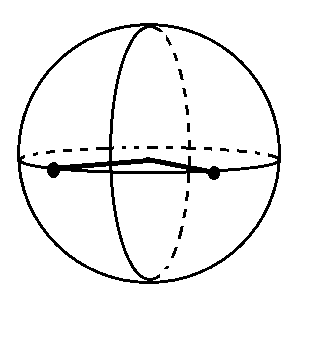
\includegraphics[width=0.3\textwidth]{Q3_c.png}
  \caption{We see our two particles on the same equitorial plane $\theta = \pi/2$, at the same radius but with possibly different $\varphi$.}
\end{figure}

\textbf{(ii)} 
\newpage
\textbf{Question 4}

\textbf{(a)} By inspection, the two obvious Killing Fields are $\partial_{t}$ and $\partial_{\varphi}$. Since we have no dependence upon $t$ in our metric, we do indeed have a stationary geometry, and hence have a symmetry in time translations. We know that time translation is associated with energy, $E$, and symmetry in $\varphi$ is conservation of an angular momentum of sorts. That is, we get the two conserved quantities to be
\[ E = k^{\mu}v_{\mu} \quad \& \quad L = s^{\mu}v_{\mu} \]
where $v \in \Gamma(TM)$ and in particular is the geodesic vector field, $k$ is the vector associated with the $t$ coordinate and $s$ is the vector associated with the $\varphi$ component. We see that
\[ E = g_{\mu\nu}k^{\mu}v^{\nu} = g_{00}k^{0}v^{0} = \left(a^{2} - \frac{\Delta}{\Sigma}\right)\frac{dt}{d\tau} \]
\[ L = g_{\mu\nu}s^{\mu}v^{\nu} = g_{33}s^{3}v^{3} = \left(-\frac{\Delta}{\Sigma}a^{2}\sin^{4}\theta + \frac{\sin^{2}\theta}{\Sigma}(r^{2} + a^{2})^{2}\right)\frac{d\varphi}{d\tau} \]

\textbf{(b)} We use the variation to see
\[ \delta S = \int_{\lambda_{0}}^{\lambda}d\lambda \delta L = \int_{\lambda_{0}}^{\lambda}d\lambda\left(\frac{\partial L}{\partial x^{\mu}}\delta x^{\mu} + \frac{\partial L}{\partial \dot{x}^{\mu}}\delta \dot{x}^{\mu} + \frac{\partial L}{\partial \lambda}\delta \lambda\right) \]
where the bounding conditions give us tha the last term vanishes. We now apply the ELE to get
\[ \delta S = \int_{\lambda_{0}}^{\lambda}d\lambda\left(\del{\lambda}\frac{\partial L}{\partial \dot{x}^{\mu}}\delta x^{\mu} + \frac{\partial L}{\partial \dot{x}^{\mu}}\del{\lambda}\delta x^{\mu}\right) \]
but applying the product rule on the second term gives us
\[ \delta S = \int_{\lambda_{0}}^{\lambda}d\lambda\left( \del{\lambda}\frac{\partial L}{\partial \dot{x}^{\mu}}\delta x^{\mu}+ \del{\lambda}\left(\frac{\partial L}{\partial \dot{x}^{\mu}}\delta x^{\mu}\right) - \del{\lambda}\frac{\partial L}{\partial \dot{x}^{\mu}}\delta x^{\mu}\right) = \int_{\lambda_{0}}^{\lambda}d\lambda\del{\lambda}\left(\frac{\partial L}{\partial \dot{x}^{\mu}}\delta x^{\mu}\right) = \frac{\partial L}{\partial \dot{x}^{\mu}}\delta x^{\mu}\]
\[ \implies \frac{\partial S}{\partial x^{\mu}} = \frac{\partial L}{\partial \dot{x}^{\mu}}\, .\]
So, taking the variation of $S$, we see
\[ \delta S = \di[S]{\lambda}\delta \lambda + \di[S]{\dot{x}^{\mu}}\delta \dot{x}^{\mu} = L\delta \lambda - \di[L]{\dot{x}^{\mu}}\dot{x}^{\mu}\delta \lambda\]
which we recognize to just be the Hamiltonian, and thus
\[ \implies \di[S]{\lambda} = -H = -\left(\di{\dot{x}^{\mu}}\left(\frac{1}{2}g_{\mu\nu}\dot{x}^{\mu}\dot{x}^{\nu}\right)\dot{x}^{\mu} - \frac{1}{2}g_{\mu\nu}\dot{x}^{\nu}\dot{x}^{\nu}\right) = g_{\mu\nu}\dot{x}^{\mu}\dot{x}^{\nu} - \frac{1}{2}g_{\mu\nu}\dot{x}^{\mu}\dot{x}^{\nu} \]
\[\di[S]{\lambda} = -\frac{1}{2}g^{\mu\nu}\di[S]{\dot{x}^{\mu}}\di[S]{\dot{x}^{\nu}} \, .\]

\textbf{(c)} We wish to find the inverse metric to the given $g_{\mu\nu}$. Notice that the metric is already in it's orthogonal form, and so we need to only find the basis vectors that make these one-forms the identity. First, by inspection we know that the first inverse basis vector will be a combination of $\partial_{\varphi}$ and $\partial_{t}$. So, we see that we need a basis vector that would go to the identity when applied to $\sqrt{\Delta/\Sigma}dt - \sqrt{\Delta/\Sigma}a \sin^{2}\theta d\varphi$, that is we need $\Upsilon^{0}$ such that
\[ \langle\Upsilon_{0},\Upsilon^{0}\rangle =  \sqrt{\Delta/\Sigma}dt\langle dt,\Upsilon^{0}\rangle - \sqrt{\Delta/\Sigma}a \sin^{2}\theta \langle d\varphi, \Upsilon^{0}\rangle = 1\]
but since we know that given coordinate basis, $\partial_{\mu}$, is orthonormal we can see that we need $\Upsilon^{0} = A\partial_{r} + B\partial_{\varphi}$. So, we get the system
\[ \sqrt{\Delta/\Sigma}A - \sqrt{\Delta/\Sigma}a \sin^{2}\theta B = 1 \]
but we also require that this be orthogonal with the other basis, which is non-trivial only for
\[ \frac{\sin\theta}{\sqrt{\Sigma}}(r^{2} + a^{2})B - a\frac{\sin \theta}{\sqrt{\Sigma}}A = 0 \]
So, we can apply elimination by multiplying the second system by $\sqrt{\Delta}/a\sin\theta$ and adding the two to get
\[ \left(\frac{\sqrt{\Delta}}{a\sqrt{\Sigma}}(r^{2} + a^{2}) - \sqrt{\Delta/\Sigma}a\sin^{2}\theta\right)B = 1 \]
\[ \implies B = \sqrt{\frac{\Sigma}{\Delta}}\frac{a}{r^{2} + a^{2}\cos^{2}\theta} = \frac{a}{\sqrt{\Sigma\Delta}} \]
\[\implies A = \frac{r^{2} + a^{2}}{a}B = \frac{r^{2} +a^{2}}{\sqrt{\Sigma\Delta}} \]
and by inspection we can 
\[\Upsilon^{1} = \sqrt{\frac{\Delta}{\Sigma}}\partial_{r} \hspace{3em} \& \hspace{3em} \Upsilon^{2} = \frac{1}{\sqrt{\Sigma}}\partial_{\theta} \, .\]
Now, we need to find $\Upsilon^{3} = C\partial_{t} + D\partial_{\varphi}$ where we get the two systems
\[ \frac{\sin\theta}{\sqrt{\Sigma}}(r^{2} + a^{2})D - a\frac{\sin\theta}{\sqrt{\Sigma}}C = 1\]
\[ \sqrt{\Delta/\Sigma}C - \sqrt{\Delta/\Sigma}a \sin^{2}\theta D = 0 \]
We use substitution to get
\[ C = a\sin^{2}\theta D \implies \left(\frac{\sin\theta}{\sqrt{\Sigma}}(r^{2} + a^{2}) - a\frac{\sin\theta}{\sqrt{\Sigma}}a\sin^{2}\theta\right)D = 1\]
\[ \implies D = \frac{\sqrt{\Sigma}}{\sin\theta}\left(\frac{1}{r^{2} + a^{2}\cos^{2}\theta}\right) = \frac{1}{\sqrt{\Sigma}\sin\theta}\]
\[\implies C = \frac{a\sin\theta}{\sqrt{\Sigma}} \]
So, we are done and our inverse metric in coordinates is
\[ g^{-1} = -\left(\frac{r^{2} +a^{2}}{\sqrt{\Sigma\Delta}}\partial_{t} + \frac{a}{\sqrt{\Sigma\Delta}}\partial_{\varphi}\right)^{2} + \frac{\Delta}{\Sigma}\partial_{r}^{2} + \frac{1}{\Sigma}\partial_{\theta}^{2} + \left(\frac{a\sin\theta}{\sqrt{\Sigma}}\partial_{t} + \frac{1}{\sqrt{\Sigma}\sin\theta}\partial_{\varphi}\right)^{2} \, .\]

\textbf{(d)}

\newpage
\textbf{Question 5}

\textbf{(a)} We need to use the metric to get $\partial_{\mu}S = u_{\mu} = g_{\nu\mu}u^{\mu}$ where $u^{\mu}$ is still the velocity, and so $u^{\mu} = \dot{x}^{\mu}$. Then, we see that
\[ \mathcal{E} = \partial_{t}S = g_{\nu t}u^{t} = g_{tt}\dot{t} + g_{\varphi t}\dot{t} \]
\[ -R' = \partial_{r}S = g_{rr}\dot{r} \hspace{3em} \& \hspace{3em} -\Lambda' = \partial_{\theta}S = g_{\theta\theta}\dot{\theta} \]
\[ \Lambda' = 
\end{document}
